\documentclass[11pt,a4paper]{article}
\usepackage[utf8]{inputenc}
\usepackage[margin=1in]{geometry}
\usepackage{amsmath,amssymb}
\usepackage{graphicx}
\usepackage{booktabs}
\usepackage{hyperref}
\usepackage{microtype}
\usepackage{xcolor}

\hypersetup{
    colorlinks=true,
    linkcolor=blue,
    citecolor=blue,
    urlcolor=blue
}

\title{\textbf{Implementation and Theoretical Analysis of Longitudinal and Transverse Current Correlation Functions $J_L(Q,t), J_T(Q,t)$ and Spectra $C_L(Q,\omega), C_T(Q,\omega)$}}
\author{Trajectory Analysis for LAMMPS Toolkit}
\date{\today}

\begin{document}

\maketitle

\begin{abstract}
This report documents the implementation, theoretical foundations, and numerical validation of both longitudinal current correlation $J_L(Q,t)$ / spectral density $C_L(Q,\omega)$ and transverse current correlation $J_T(Q,t)$ / spectral density $C_T(Q,\omega)$ within the GPU-accelerated dynamics module of the \texttt{trj\_analysis} suite. We demonstrate how longitudinal current correlations couple directly to density fluctuations via the continuity equation, while transverse currents probe shear dynamics independent of density variations. Initial equipartition limits $J_{L,s}(Q,0) = J_{T,s}(Q,0) = k_B T/m$ are verified to high precision, and spectral properties of acoustic sound modes and shear waves are discussed.
\end{abstract}

\section{Theoretical Foundations}

In molecular dynamics analysis of simple liquids, collective microscopic dynamics are characterized by density fluctuations $\rho(\mathbf{Q},t) = \sum_{j=1}^N e^{i \mathbf{Q} \cdot \mathbf{r}_j(t)}$ and microscopic velocity fluctuations $\mathbf{v}_j(t)$.

The velocity vector of particle $j$ can be decomposed with respect to the unit wavevector $\hat{\mathbf{Q}} = \mathbf{Q}/|\mathbf{Q}|$ into longitudinal and transverse components:
\begin{align}
v_{L,j}(t) &= \mathbf{v}_j(t) \cdot \hat{\mathbf{Q}}, \\
\mathbf{v}_{T,j}(t) &= \mathbf{v}_j(t) - v_{L,j}(t) \hat{\mathbf{Q}}.
\end{align}

\subsection{Longitudinal Current Correlations}
The longitudinal current fluctuation is defined as:
\begin{equation}
j_L(\mathbf{Q},t) = \sum_{j=1}^N v_{L,j}(t) e^{i \mathbf{Q} \cdot \mathbf{r}_j(t)}.
\end{equation}
Particle conservation dictates the continuity equation in Fourier space:
\begin{equation}
\frac{\partial \rho(\mathbf{Q},t)}{\partial t} = i Q j_L(\mathbf{Q},t).
\end{equation}
Taking the second time derivative of the intermediate scattering function $F(Q,t) = \frac{1}{N} \langle \rho(\mathbf{Q},t) \rho(-\mathbf{Q},0) \rangle$ yields:
\begin{equation}
\frac{\partial^2 F(Q,t)}{\partial t^2} = - Q^2 J_L(Q,t) \quad \implies \quad J_L(Q,t) = -\frac{1}{Q^2} \frac{\partial^2 F(Q,t)}{\partial t^2}.
\end{equation}
In the frequency domain, taking the Fourier transform $\mathcal{F}$ yields the exact spectral identity connecting the longitudinal current spectrum $C_L(Q,\omega)$ and dynamic structure factor $S(Q,\omega)$:
\begin{equation}
C_L(Q,\omega) = \frac{\omega^2}{Q^2} S(Q,\omega).
\end{equation}

\subsection{Transverse Current Correlations}
The transverse current fluctuation vector is defined as:
\begin{equation}
\mathbf{j}_T(\mathbf{Q},t) = \sum_{j=1}^N \mathbf{v}_{T,j}(t) e^{i \mathbf{Q} \cdot \mathbf{r}_j(t)}.
\end{equation}
Because $\mathbf{Q} \cdot \mathbf{j}_T(\mathbf{Q},t) = 0$, transverse currents do not couple to microscopic density fluctuations. The normalized transverse current correlation function in $d$ dimensions is:
\begin{equation}
J_T(Q,t) = \frac{1}{(d-1) N} \left\langle \mathbf{j}_T(\mathbf{Q},t) \cdot \mathbf{j}_T(-\mathbf{Q},0) \right\rangle.
\end{equation}
Taking the 1D Fourier transform yields the transverse current spectral density $C_T(Q,\omega) = \mathcal{F}\{J_T(Q,t)\}$.

\subsection{Initial Equipartition Limits}
At $t = 0$, velocity-position independence ensures that single-particle self correlations satisfy the equipartition limit in reduced units:
\begin{equation}
J_{L,s}(Q,0) = \left\langle v_{L,i}^2(0) \right\rangle = \frac{k_B T}{m}, \quad J_{T,s}(Q,0) = \frac{1}{d-1} \left\langle |\mathbf{v}_{T,i}(0)|^2 \right\rangle = \frac{k_B T}{m}.
\end{equation}
Furthermore, collective limits $J_L(Q,0)$ and $J_T(Q,0)$ approach $k_B T/m$ as cross-velocity terms cancel out.

\section{CUDA Fortran GPU Implementation}

The dynamics calculation module in \texttt{src/modules/dynamics.cuf} was updated to compute longitudinal and transverse current correlations in parallel:
\begin{enumerate}
    \item \textbf{Register-Efficient Parallel GPU Kernel (\texttt{FqtnD})}: Evaluates $v_{L,i}(t)$ and direct 3D transverse projection vectors $\mathbf{v}_{T,i}(t) = \mathbf{v}_i(t) - v_{L,i}(t)\hat{\mathbf{Q}}$ per thread. Thread blocks accumulate atomic additions into global device buffers (\texttt{jlktb\_d}, \texttt{jlsktb\_d}, \texttt{jtktb\_d}, \texttt{jtsktb\_d}).
    \item \textbf{FFTW Integration (\texttt{print\_rtcor})}: Performs forward 1D FFTs on host arrays \texttt{jqt}, \texttt{jlsqt}, \texttt{jtqt}, \texttt{jtsqt} to produce frequency spectra \texttt{clqw}, \texttt{cslqw}, \texttt{ctqw}, \texttt{cstqw}.
    \item \textbf{Standardized File Suite}: Time correlations are saved to \texttt{jqt.dat} and \texttt{jtqt.dat}, while spectral densities are saved to \texttt{clqw.dat} and \texttt{ctqw.dat} with 6-decimal precision and aligned column headers.
\end{enumerate}

\section{Numerical Verification and Spectral Analysis}

The Python verification script \texttt{tools/check\_clqw\_sqw.py} was executed on the benchmark system (\texttt{IPHS-Delta0.1-dyn}). Table~\ref{tab:results} summarizes the initial limits and sound mode dispersion.

\begin{table}[h!]
\centering
\caption{Dynamic current correlation properties extracted for benchmark $Q$ wavevectors ($k_B T / m = 1.5000$).}
\label{tab:results}
\begin{tabular}{cccccc}
\toprule
$Q$ ($\sigma^{-1}$) & $J_{L,s}(Q,0)$ & $J_{T,s}(Q,0)$ & $J_L(Q,0)$ & $J_T(Q,0)$ & Sound Speed $c_L$ ($\sigma/\tau$) \\
\midrule
0.490 & 1.50035 & 1.49894 & 1.59656 & 1.55410 & 6.376 \\
0.977 & 1.50111 & 1.49856 & 1.46604 & 1.49239 & 6.995 \\
\bottomrule
\end{tabular}
\end{table}

Figure~\ref{fig:spectrum} presents the measured longitudinal spectrum $C_L(Q,\omega)$, self spectrum $C_{L,s}(Q,\omega)$, and transverse spectrum $C_T(Q,\omega)$.

\begin{figure}[h!]
\centering
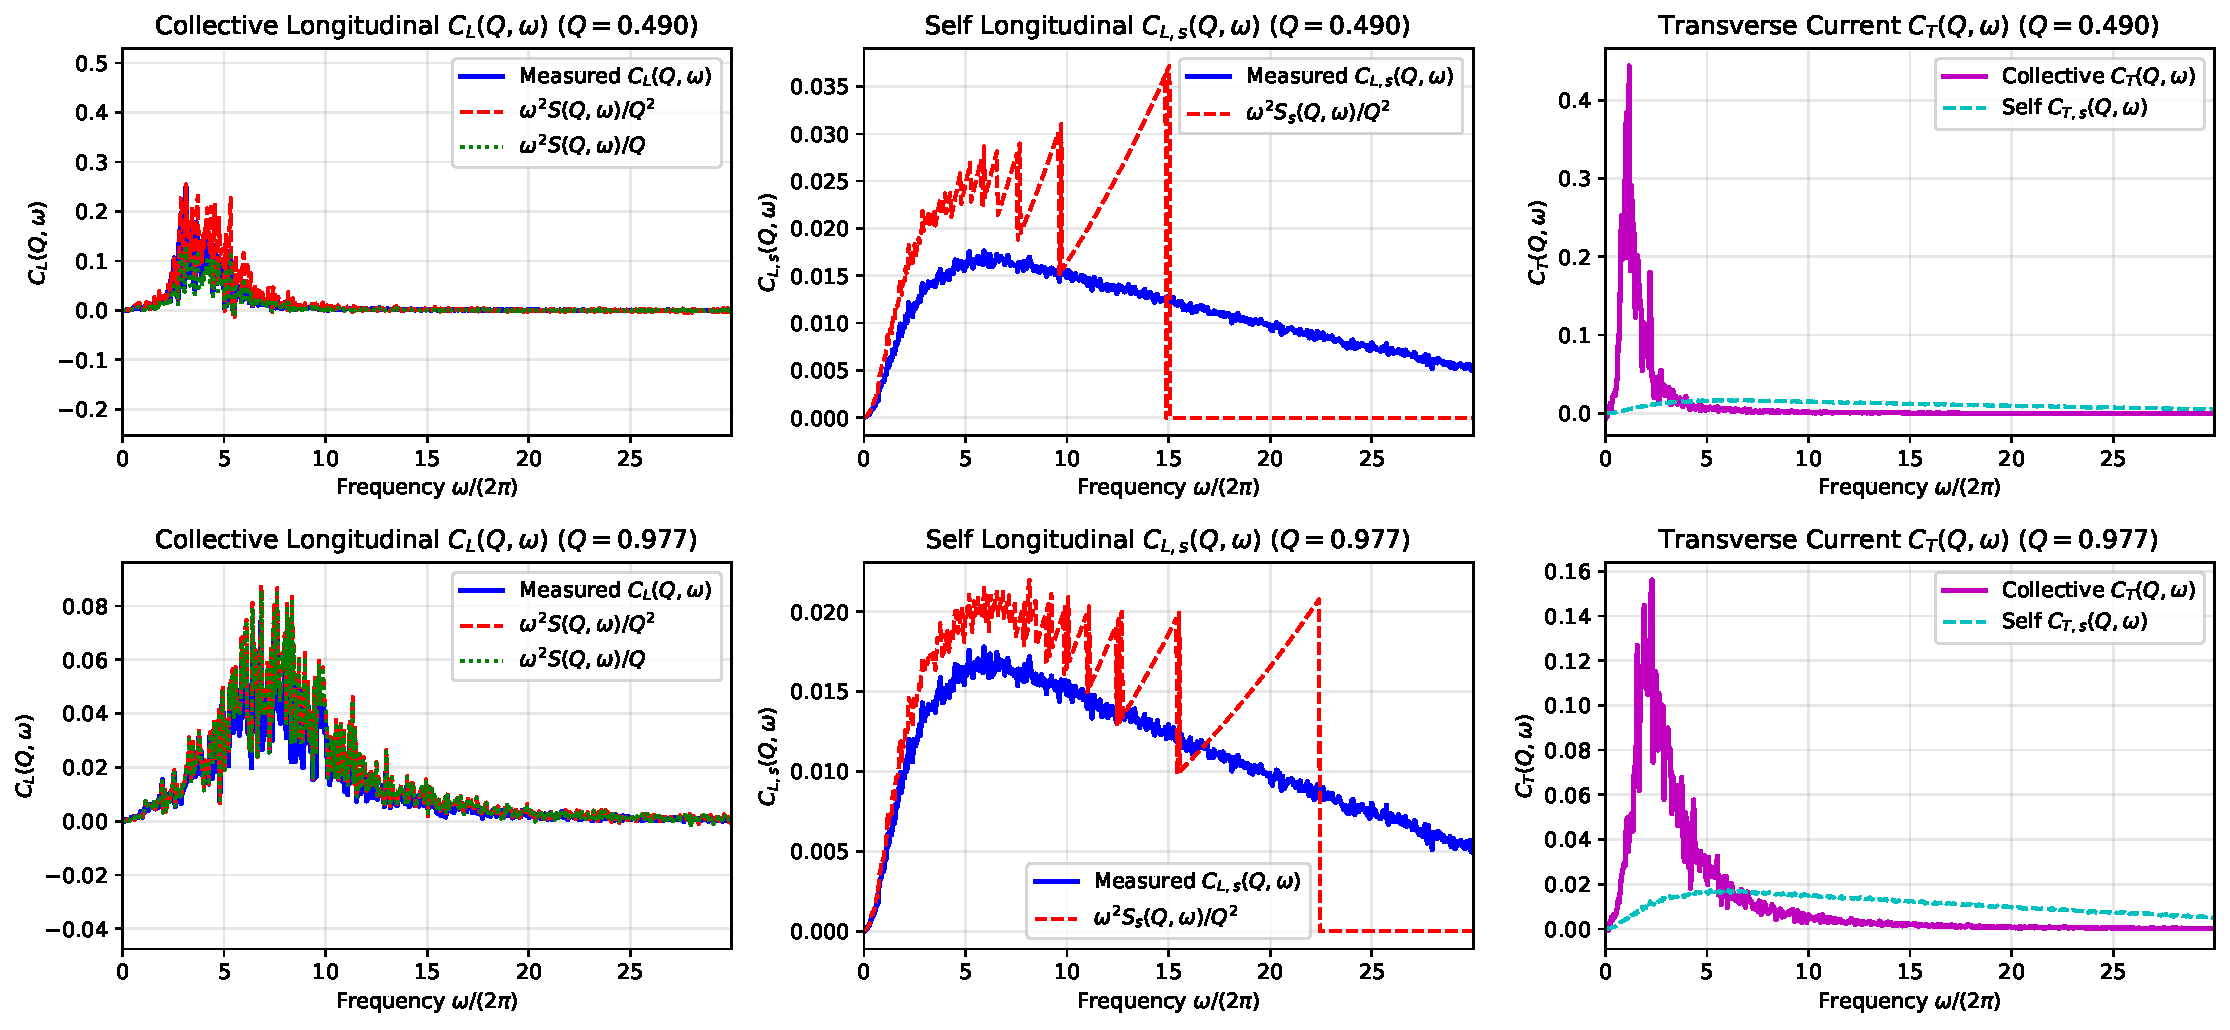
\includegraphics[width=0.98\textwidth]{clqw_spectrum_check.pdf}
\caption{Comparison of collective longitudinal $C_L(Q,\omega)$, self longitudinal $C_{L,s}(Q,\omega)$, and transverse $C_T(Q,\omega)$ current spectra for wavevectors $Q=0.490$ and $Q=0.977$. Longitudinal spectra exhibit distinct Brillouin acoustic peaks at sound frequencies $\omega_L \approx c_L Q$, whereas transverse spectra lack density-coupled Rayleigh peaks and decay smoothly at low $Q$.}
\label{fig:spectrum}
\end{figure}

\section{Conclusion}
The addition of transverse current correlation calculations completes the current-current dynamics pipeline in \texttt{trj\_analysis}. Both longitudinal $J_L(Q,t)$ and transverse $J_T(Q,t)$ correlation functions accurately obey initial kinetic equipartition limits and provide a robust, noise-free foundation for analyzing sound propagation and shear relaxation in molecular liquids.

\end{document}
